\newcommand{\econtexRoot}{.}
% The \commands below are required to allow sharing of the same base code via Github between TeXLive on a local machine and ShareLaTeX.  This is an ugly solution to the requirement that custom LaTeX packages be accessible, and that ShareLaTeX seems to ignore symbolic links (even if they are relative links to valid locations)
\providecommand{\econtex}{\econtexRoot/texmf-local/tex/latex/econtex}
\providecommand{\econtexSetup}{\econtexRoot/texmf-local/tex/latex/econtexSetup}
\providecommand{\econtexShortcuts}{\econtexRoot/texmf-local/tex/latex/econtexShortcuts}
\providecommand{\econtexBibMake}{\econtexRoot/texmf-local/tex/latex/econtexBibMake}
\providecommand{\econtexBibStyle}{\econtexRoot/texmf-local/bibtex/bst/econtex}
\providecommand{\notes}{\econtexRoot/texmf-local/tex/latex/handout}
\providecommand{\handoutSetup}{\econtexRoot/texmf-local/tex/latex/handoutSetup}
\providecommand{\handoutShortcuts}{\econtexRoot/texmf-local/tex/latex/handoutShortcuts}
\providecommand{\handoutBibMake}{\econtexRoot/texmf-local/tex/latex/handoutBibMake}
\providecommand{\handoutBibStyle}{\econtexRoot/texmf-local/bibtex/bst/handout}

  

\documentclass{beamer}
\usepackage{etoolbox}
\usepackage{comment}
\usepackage{graphicx}
%\usepackage{dtklogos}
\usepackage{dsfont}
\usepackage{amsmath,amssymb}
\usepackage{\econtexShortcuts}
\usepackage[english]{babel}
\usepackage[svgnames,hyperref]{}
\usepackage{empheq}
\usepackage[many]{tcolorbox}
\usepackage{remreset}
\usepackage{tikz} 
\usetikzlibrary{tikzmark,fit,shapes.geometric}
\usetikzlibrary{tikzmark,calc,arrows,shapes,decorations.pathreplacing}
\tikzset{every picture/.style={remember picture}}
\usepackage{cancel}
\usepackage{booktabs,natbib}
\setbeamercovered{invisible}

\usepackage{dcolumn}

\tcbset{highlight math style={enhanced,
		colframe=red!60!black,colback=yellow!50!white,arc=4pt,boxrule=1pt,
}}


\makeatletter
\@removefromreset{subsection}{section}
\patchcmd{\beamer@part}{\setcounter{subsection}{0}}{}{}
\makeatother
\setcounter{subsection}{1}
\setbeamercovered{transparent}
\setbeamertemplate{navigation symbols}{}%remove navigation symbols
\begin{comment}
\setbeamertemplate{footline}
{
	\hbox{\begin{beamercolorbox}[wd=1\paperwidth,ht=2.25ex,dp=1ex,right]{framenumber}%
			\usebeamerfont{framenumber}\insertframenumber{} \hspace*{2ex}
	\end{beamercolorbox}}%
	\vskip0pt%
}
\end{comment}


\mode<presentation>{}
%% preamble
\title[Monetary Policy with Many Agents]{Monetary Policy with Many Agents}
\author{Edmund Crawley and Seungcheol Lee}
%\date[08/11/2018]{Towson University\\ November 8, 2018}
\date[09/13/2019]{}
\usetheme{Frankfurt}

\setbeamertemplate{navigation symbols}{}
\makeatletter
\setbeamertemplate{footline}
{%
	\hbox{\begin{beamercolorbox}[wd=1\paperwidth,ht=2.25ex,dp=1ex,right]{framenumber}%
		\usebeamerfont{framenumber}\insertframenumber{} \hspace*{2ex}
	\end{beamercolorbox}}%
	\vskip0pt%
	\pgfuseshading{beamer@barshade}%
	\ifbeamer@sb@subsection%
	\vskip-9.75ex%
	\else%
	\vskip-7ex%
	\fi%
	\begin{beamercolorbox}[ignorebg,ht=2.25ex,dp=3.75ex]{section in head/foot}
		\insertnavigation{\paperwidth}
	\end{beamercolorbox}%
	\ifbeamer@sb@subsection%
	\begin{beamercolorbox}[ignorebg,ht=2.125ex,dp=1.125ex,%
		leftskip=.3cm,rightskip=.3cm plus1fil]{subsection in head/foot}
		\usebeamerfont{subsection in head/foot}\insertsubsectionhead \insertframenumber{} \hspace*{2ex}
	\end{beamercolorbox}%
	\fi%
}%
\setbeamertemplate{headline}{%
}
\makeatother
\begin{document}
\setbeamertemplate{caption}{\raggedright\insertcaption\par}
\newcolumntype{d}[1]{D{.}{.}{#1}}
%circled draws a circle around a number
\newcommand*\circled[1]{\tikz[baseline=(char.base)]{
		\node[shape=circle,draw,inner sep=2pt] (char) {#1};}}

\begin{frame}[plain]
\titlepage
\end{frame}
\addtocounter{framenumber}{-1}
\section{Motivation}
\setbeamercovered{invisible}
\frame
{
	\frametitle{How do interest rate changes affect consuption behavior?}
	Standard New Keynesian Theory $\implies$ Intertemporal Substitution
	\vspace{0.5cm}
	\pause
	\begin{columns}
	\column{0.5\linewidth}
	\centering
	\textcolor{blue}{Recent Theory} \\
	Income and Redistribution \\
	Effects are Large
	\column{0.5\linewidth}
\pause
	\centering
	\textcolor{blue}{Recent Empirics} \\
	Income and Redistribution \\
	Effects are Large
	\end{columns}
\pause
\vspace{0.5cm}
	\centering
	BUT - the mechanisms are very different
}

\frame
{
	\frametitle{How do interest rate changes affect consuption behavior?}
	\textcolor{blue}{Recent Theory (HANK)}
	\begin{itemize}
	\item Countercyclical profits and govt redistribution play large role
	\item No private debt
	\end{itemize}
	\textcolor{blue}{Recent Empirics} 
	\begin{itemize}
	\item Unhedged interest rate exposure 
	\item Income sensitivity to business cycles
	\end{itemize}
	\vspace{0.5cm}
	This paper - attempt to bring models closer to empirics
}
\frame[t]
{
	\frametitle{Some Motivation from Denmark}
	\only<1>{
		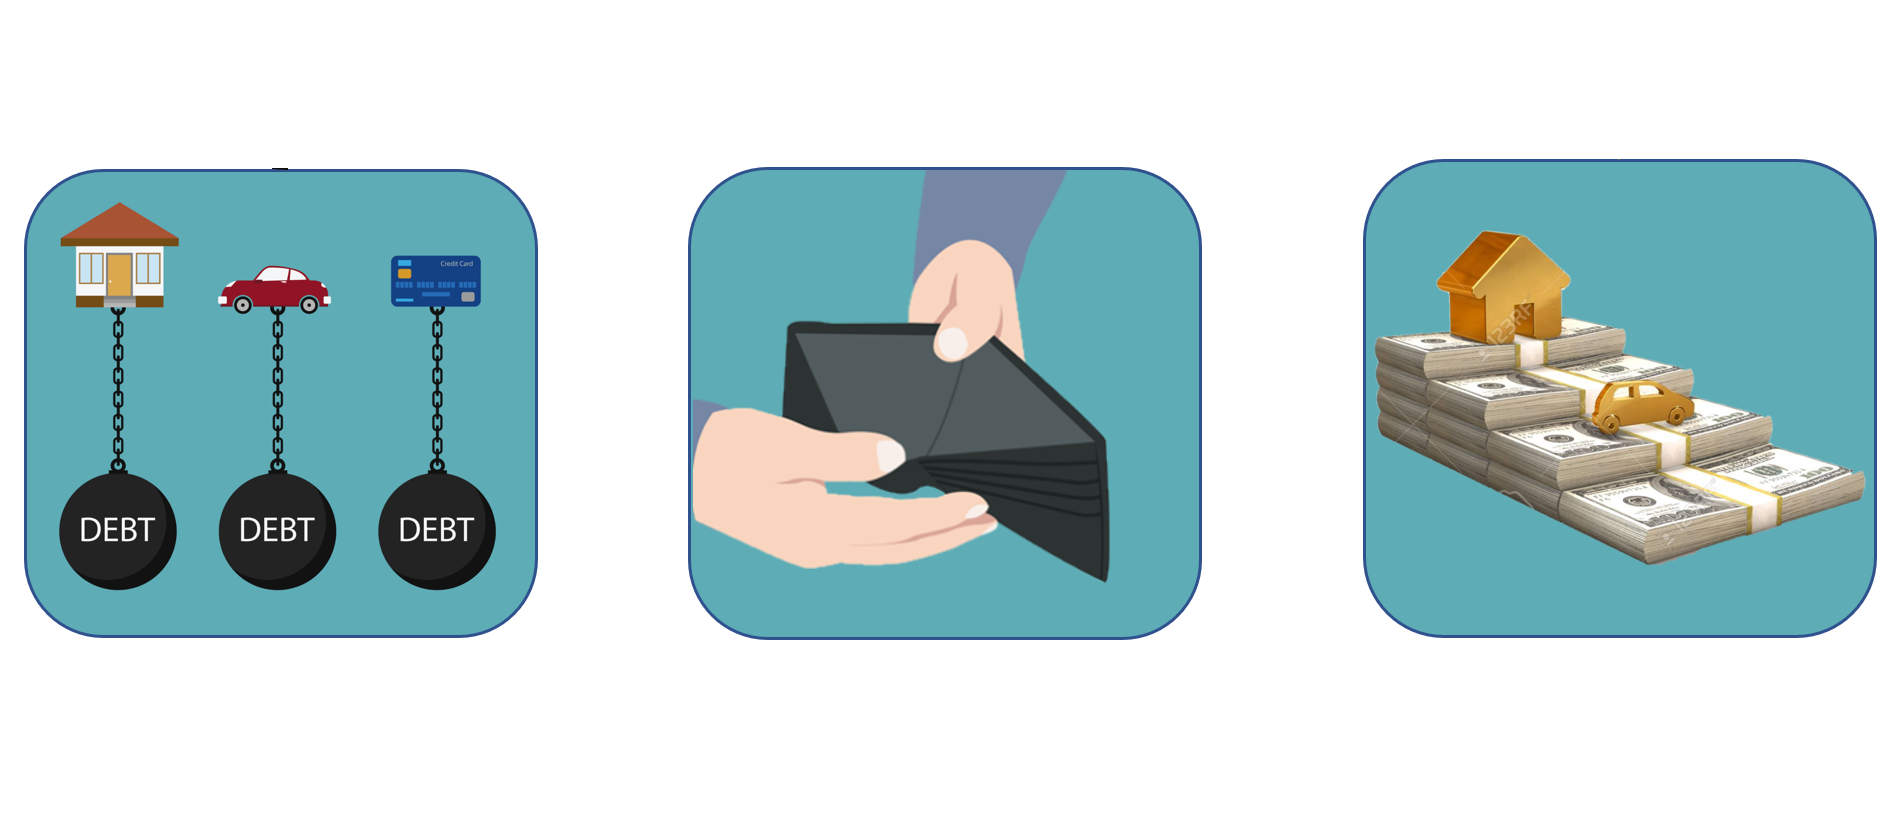
\includegraphics[width=11cm]{IRE_Big1.png}
	}
	\only<2>{
		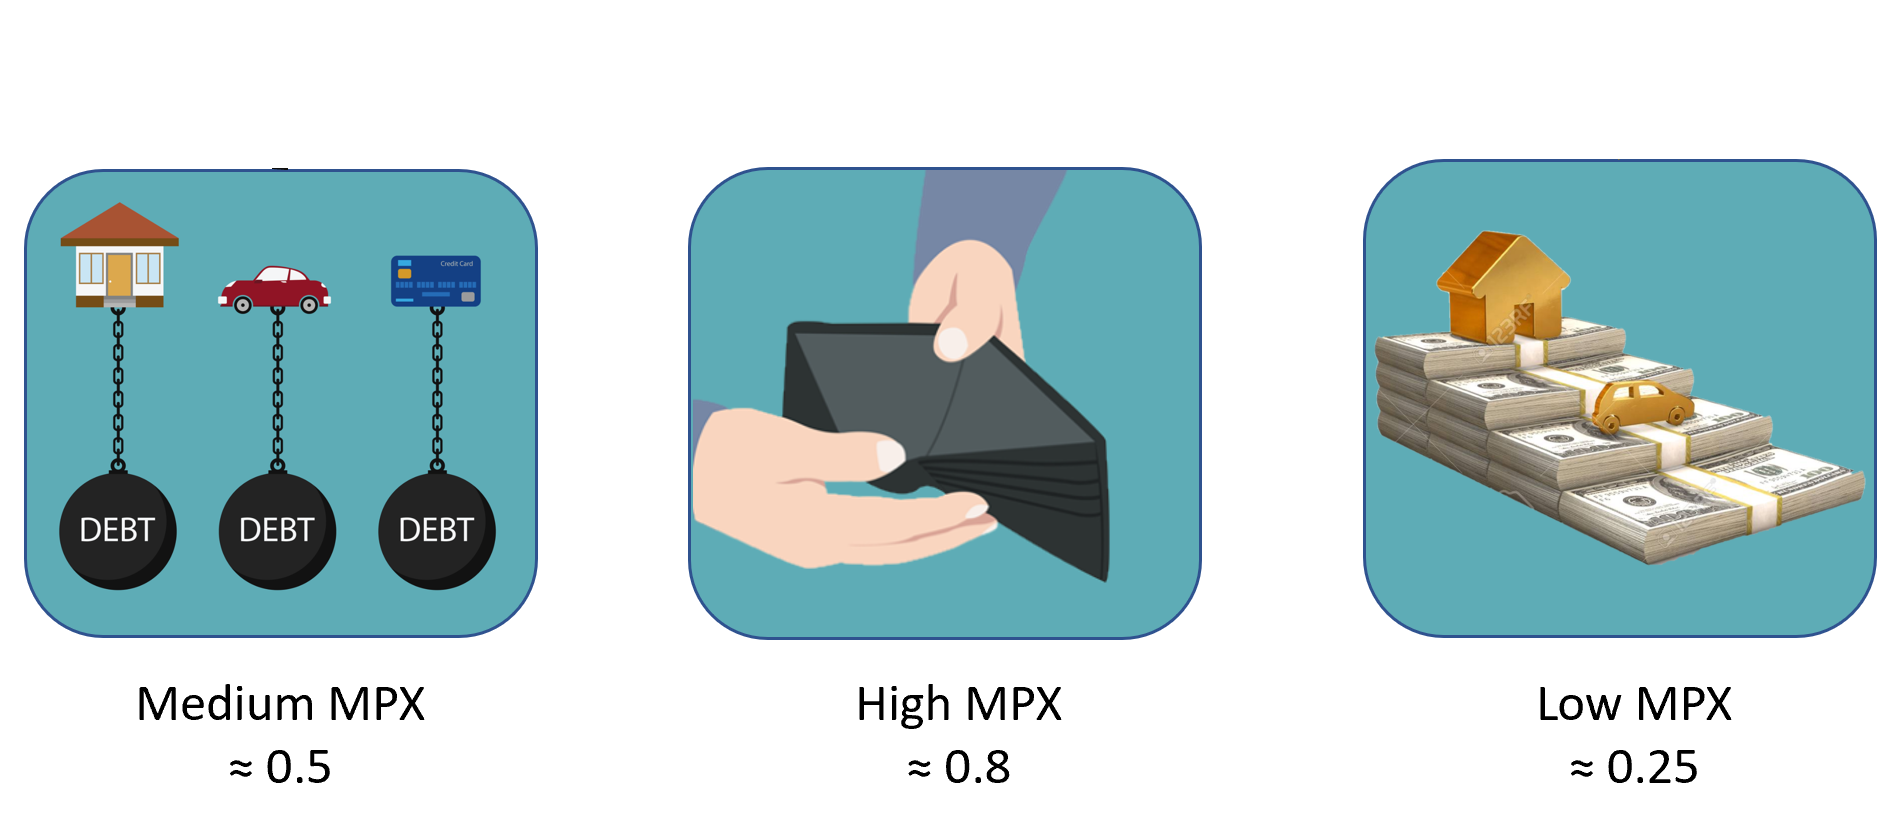
\includegraphics[width=11cm]{IRE_Big2.png}
		\\[0.7cm]
		MPX: Marginal Propensity to eXpend (includes durables)
	}
	\only<3->{
		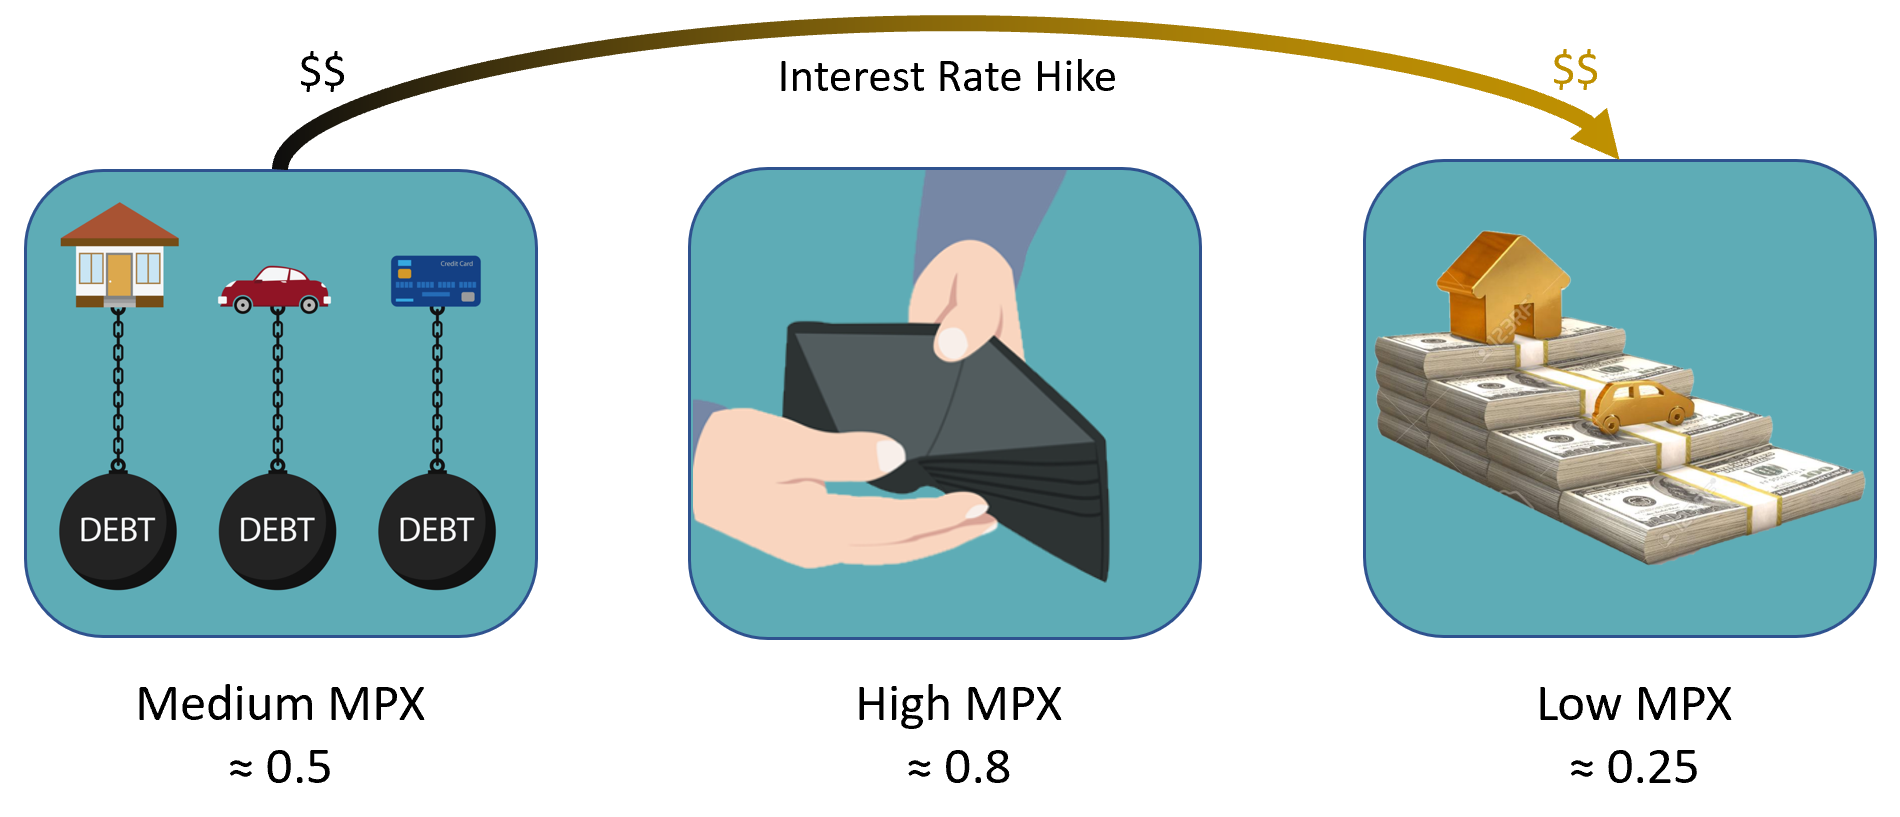
\includegraphics[width=11cm]{IRE_Big3.png} \tikz[baseline]{\node(ire){}}
	}
	\only<3>{
		\begin{tikzpicture}[remember picture,overlay]
		\node (ire1a)  at ([shift={(-9.5,0.0)}]ire) {};
		\node (ire1b)  at ([shift={(-0.4,-0.4)}]ire1a) {};
		\draw[blue,thick,->] (ire1a)  to [in=45,out=225] (ire1b) node[anchor=north,text = blue] {\begin{tabular}{l} Decrease spending \\ a \textit{lot}  \end{tabular}};
		\node (ire1c)  at ([shift={(-1.5,0.0)}]ire) {};
		\node (ire1d)  at ([shift={(0.4,-0.4)}]ire1c) {};
		\draw[blue,thick,->] (ire1c)  to [in=135,out=315] (ire1d) node[anchor=north,text = blue] {\begin{tabular}{r} Increase spending \\ a \textit{little}  \end{tabular}};
		\end{tikzpicture}
	}
	\only<4->{
		\vspace{-.5cm}
		\begin{align*}
		\text{1yr rate }&\uparrow \ 1\% \\
		\tikz[baseline]{\node(aggregate){}} \textit{Aggregate}\text{ Spending }&\downarrow \ 26 \text{ basis points}
		\end{align*}
		\begin{tikzpicture}[remember picture,overlay]
		\node (aggregatea)  at ([shift={(1.5,-0.1)}]aggregate) {};
		\node (aggregateb)  at ([shift={(-0.4,-0.4)}]aggregatea) {};
		\draw[blue,thick,->] (aggregatea)  to [in=45,out=225] (aggregateb) node[anchor=north,text = blue] {Through this redistribution channel \textit{alone}};
		\end{tikzpicture}
	}
}
\frame{
	\frametitle{Auclert's Decomposition}
	How does Monetary Policy Effect Aggregate Consumption?\\
	\bigskip
	\begin{itemize}
		\item Intertemporal Substitution \tikz[baseline]{\node(topbrace1){}}
		\item Aggregate Income \tikz[baseline]{\node(bottombrace1){}}
		\begin{tikzpicture}[overlay, remember picture]
		\draw [decoration={brace,amplitude=0.5em},decorate,ultra thick,black]
		let \p1=(topbrace1), \p2=(bottombrace1) in
		({max(\x1,\x2)+1.8em}, {\y1+0.8em}) -- node[right=0.6em] {Representative Agent Channels} ({max(\x1,\x2)+1.8em}, {\y2});
		\end{tikzpicture}
		\pause
		\only<2>{
			\begin{tikzpicture}[remember picture,overlay]
			\node (topbrace1a)  at ([shift={(-5,0.1)}]topbrace1) {};
			\node (topbrace1b)  at ([shift={(-5,1.8)}]topbrace1) {};
			\node (bottombrace1a)  at ([shift={(-3.7,0.1)}]bottombrace1) {};
			\node (bottombrace1b)  at ([shift={(-3.7,-0.7)}]bottombrace1) {};
			\draw[blue,thick,->] (topbrace1a)  to [in=180,out=180] (topbrace1b) node[anchor=west,text = blue] {Dominates in Rep. Agent NK models};
			\draw[blue,thick,->] (bottombrace1a)  to [in=180,out=180] (bottombrace1b) node[anchor=west,text = blue] {Large in Spender-Saver, or TANK models};
			\end{tikzpicture}
		}
		\pause
		\item Fisher (Inflationary debt relief) \tikz[baseline]{\node(topbrace2){}}
		\item Earnings Heterogeneity
		\item Interest Rate Exposure \tikz[baseline]{\node(m1){}}
		\begin{tikzpicture}[overlay, remember picture]
		\draw [decoration={brace,amplitude=0.5em},decorate,ultra thick,black]
		let \p1=(topbrace2), \p2=(m1) in
		({max(\x1,\x2)}, {\y1+0.8em}) -- node[right=0.6em] {Redistribution Channels} ({max(\x1,\x2)}, {\y2});
		\end{tikzpicture}
	\end{itemize}
}
\section{TANK}
\frame
{
	\frametitle{Two Agent New Keynesian Models (TANK)}
	\begin{itemize}
		\item Simplest Model with Redistribution Channels
		\item Widely used by Policy Institutions (esp. for Fiscal Policy)
		\item Many insights carry over to HANK models
	\end{itemize}
\bigskip
\pause
Two Agents: Ricardian and Keynesian\\
Fixed Capital (owned by Ricardian's)\\
Keynesians can borrow up to $\Omega$ of their steady state income as short term nominal bonds $\rightarrow$ Not a common feature of these models\\
Standard New Keynesian Phillips curve
}

\begin{comment}
\frame
{
	\frametitle{TANK Setup: Ricardian Households}
	Ricardian Housholds maximize:
	\begin{align*}
	\mathbb{E}\sum_{t=0}^{\infty}\beta^t \left(\frac{\left(C^R_t\right)^{1-\sigma}}{1-\sigma} - \frac{\left(N^R_t\right)^{1+\psi}}{1+\psi}\right)
	\end{align*}
	subject to budget constraint
	\begin{align*}
	P_t C^R_t + I_{t}^{-1}B_{t+1} =  N^R_t W_t + P_t D_t + B_t
	\end{align*}
	\pause
	They choose consumption by their Euler Equation:
	\begin{align*}
	\left(C^R_t\right)^{-\sigma} = \beta \mathbb{E}\left(I_t\frac{P_{t}}{P_{t+1}} \left(C^R_{t+1}\right)^{-\sigma}\right)	
	\end{align*}
}
\frame
{
	\frametitle{TANK Setup: Keynesian Households}
	Each period Keynesian Housholds maximize:
	\begin{align*}
	\frac{\left(C^K_t\right)^{1-\sigma}}{1-\sigma} - \frac{\left(N^K_t\right)^{1+\psi}}{1+\psi}\
	\end{align*}
	subject to their budget constraint:
	\begin{align}
	C^K_t \leq N^K_t \frac{W_t}{P_t} + \left(I_{t}^{-1} \frac{\mathbb{E}_t P_{t+1}}{P_t} -  \frac{\mathbb{E}_{t-1}P_t }{P_t}\right)\Omega \bar{N_K}\overline{W/P}  
	\end{align}
}
\frame
{
	\frametitle{Household Aggregation and Wage Schedule}
With the Keynesian proportion of households equal to $\lambda$, total consumption is:
\begin{align*}
C_t = \lambda C^K_t + (1-\lambda) C^R_t
\end{align*}
Hours are equally rationed between both types of household such that:
\begin{align*}
N_t = N^K_t = N^R_t
\end{align*}
The real wage is set according to the demand schedule:
\begin{align*}
\frac{W_t}{P_t} = \mathcal{M}^{\omega} \left(C_t\right)^{\sigma}\left(N_t\right)^{\psi} 
\end{align*}
}
\frame{
\frametitle{Final Goods Firms}
The final goods firm produces a final consumption good, $Y_t$, from intermediated inputs, $X_t(j)$ for $j \in [0,1]$ using the technology:
\begin{align*}
Y_t = \left( \int_0^1 X_t(j)^{1-\frac{1}{\varepsilon}} dj \right)^{\frac{\varepsilon}{\varepsilon-1}}
\end{align*}
Profit maximization yields the demand schedule $X_t(j) = \left(\frac{P_t(j)}{P_t}\right)^{-\varepsilon}$ where $P_t$ is the price of the final good. Competition also imposes a zero profit condition that yields $P_t = \left(\int_0^1 P_t^{1-\varepsilon}\right)^{\frac{1}{1-\varepsilon}}$.
}
\frame{
	\frametitle{Intermediate Goods Firms}
	Technology:
	\begin{align*}
	X_t(j) = A K_t(j)^\alpha N_t(j)^{1-\alpha}
	\end{align*}
	Calvo Fairy: Adjust price with probability $1-\theta$ \\
	\bigskip
	Leads to standard New Keynesian Phillips curve:
	\begin{align*}
	\pi_t=\beta \mathbb{E}_t\pi_{t+1}+\frac{(1-\theta)(1-\beta\theta)}{\theta}\left(\sigma +  \frac{\psi + \alpha}{1-\alpha} \right)\tilde{y}_t 
	\end{align*}
}
\frame{
	\frametitle{Monetary Policy and Equilibrium}
	Taylor Rule
	\begin{align*}
	i_t = \phi_{\pi} \pi_t + \nu_t
	\end{align*}
	\pause
	Equilibrium conditions:
	\begin{align*}
	Y_t = C_t	\label{agg_prod}
	\end{align*}
	and the total capital and labor used must equal that available:
	\begin{align*}
	\int_0^1 K_t(j)dj = \bar{K}\\
	\int_0^1 N_t(j)dj = N_t
	\end{align*}
}
\frame{
\frametitle{Calibration}
\input calib_table.tex
}
\frame{
	\frametitle{Model Fits Auclert's Transitory Framework}
	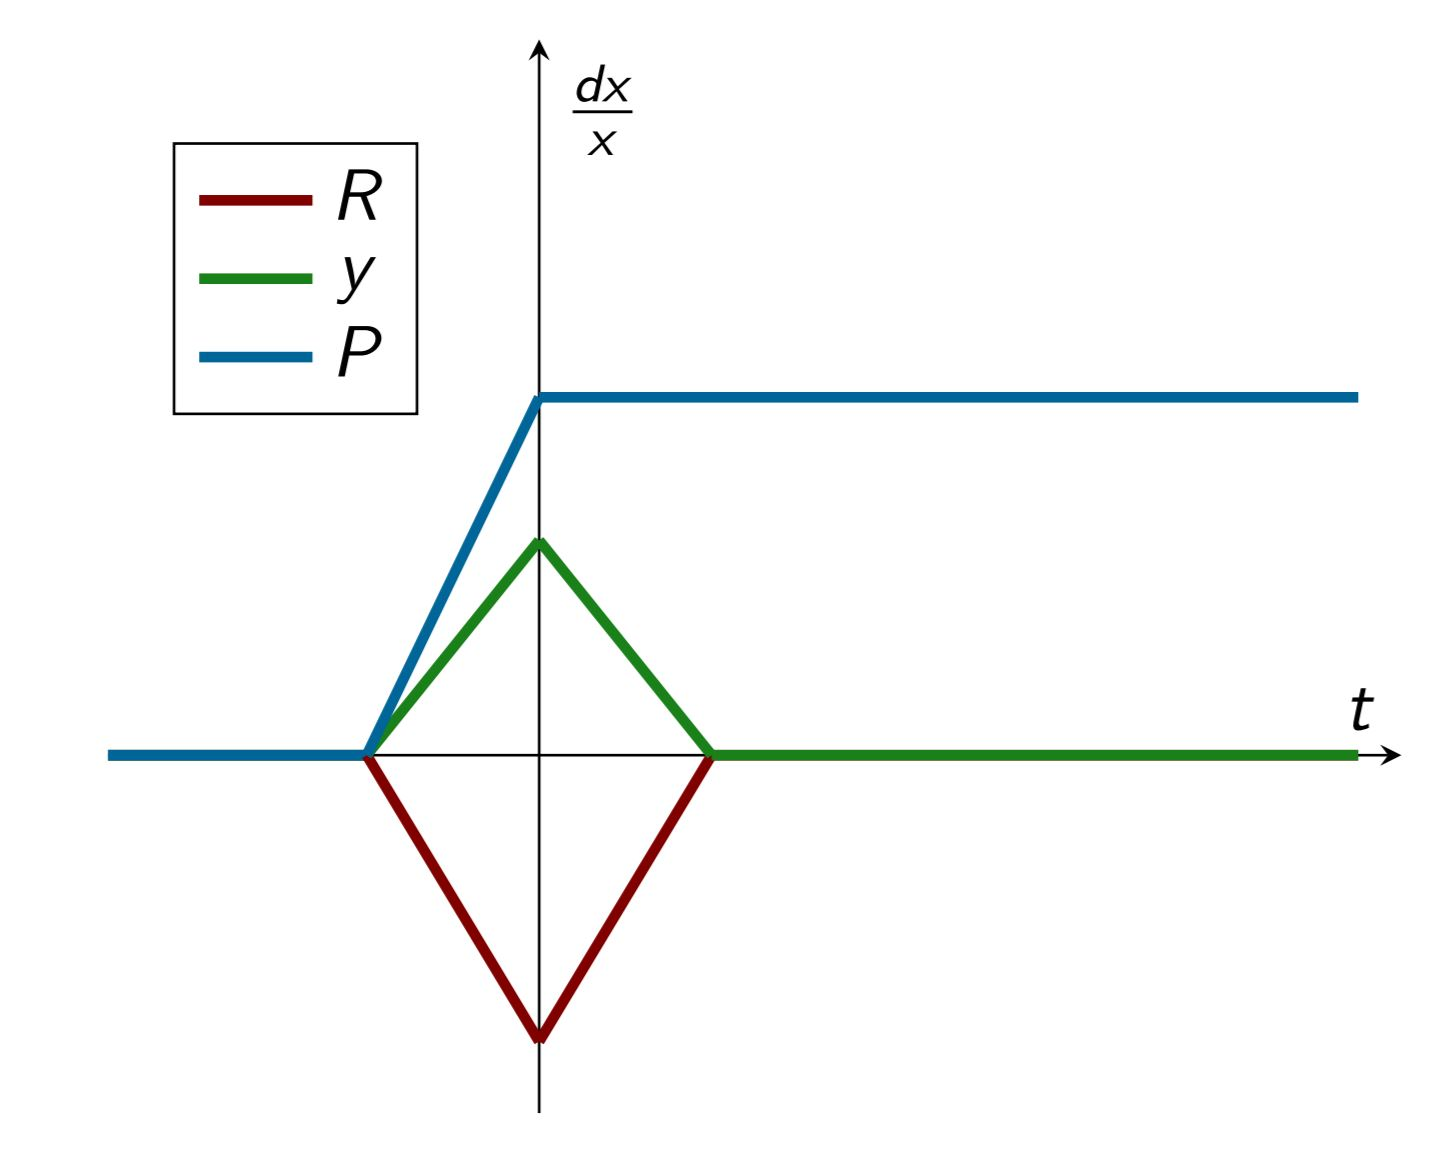
\includegraphics[width=7cm]{auclert_graph.jpg}\\
	Why? No \textit{predetermined} variables
}
\end{comment}
\frame{
	\frametitle{Model with no Debt ($\Omega=0$) and Sticky Prices}
	\centering
	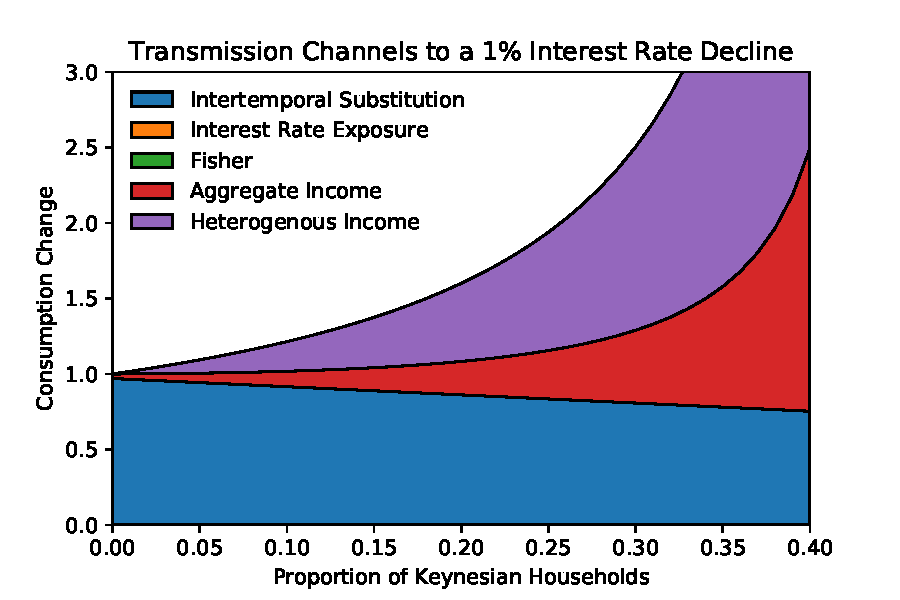
\includegraphics[scale=0.7]{ProportionKeynesian_sigma1.pdf}
}
\frame{
	\frametitle{Model with no Debt ($\Omega=0$) and Sticky Wages}
	\centering
	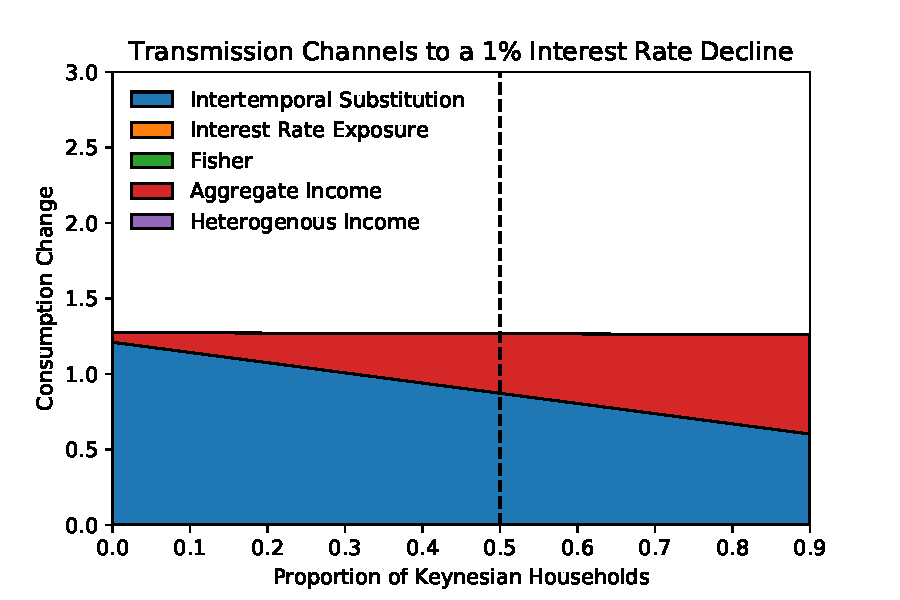
\includegraphics[scale=0.7]{ProportionKeynesian_sigma1_sw.pdf}
}
\frame{
	\frametitle{Adding Debt}
	\centering
	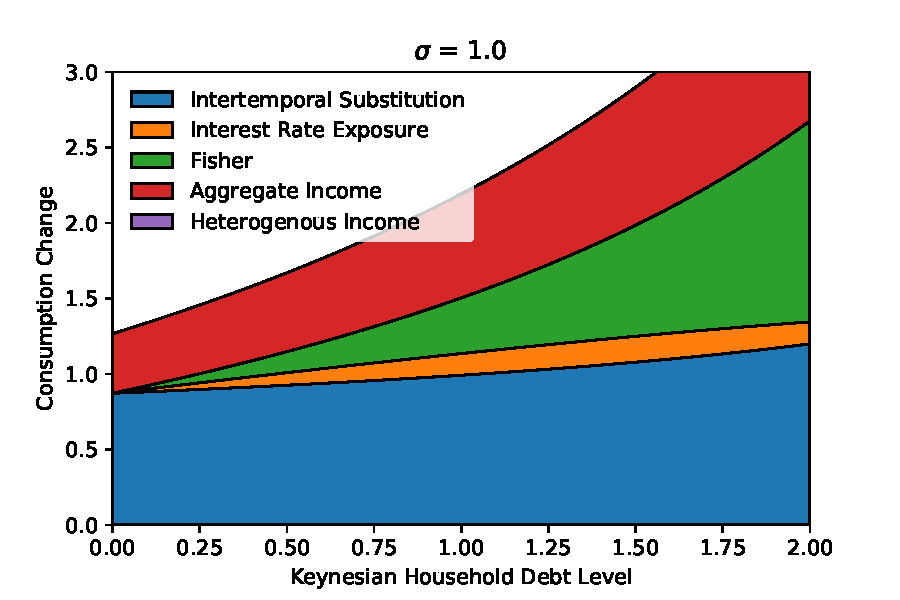
\includegraphics[scale=0.7]{KeynesianDebt_sigma1_sw.pdf}
}
\frame{
	\frametitle{Elasticity of Intertemporal Subs.}
	\centering
	\only<1>{
		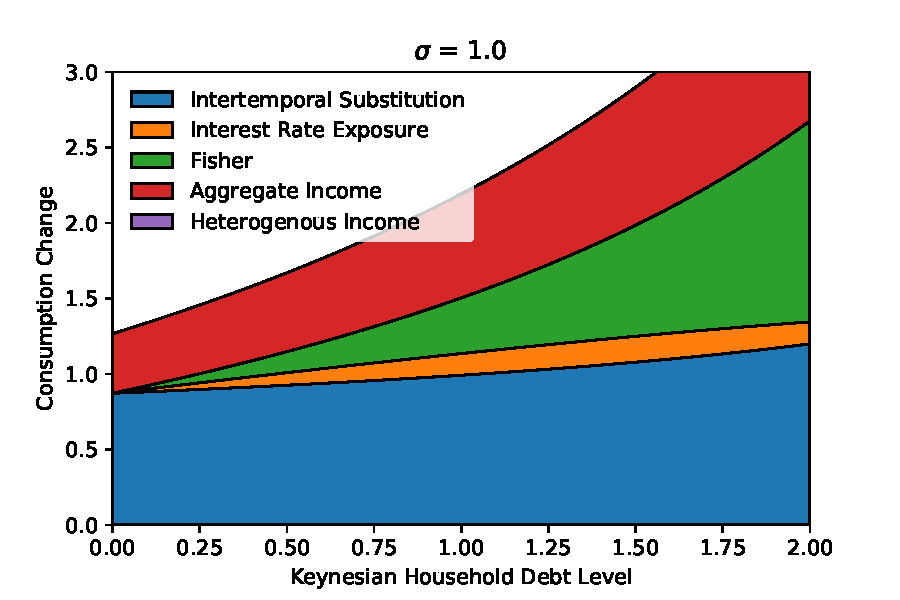
\includegraphics[width=9cm]{KeynesianDebt_sigma1_sw.pdf}\\
	}
	\only<2>{
		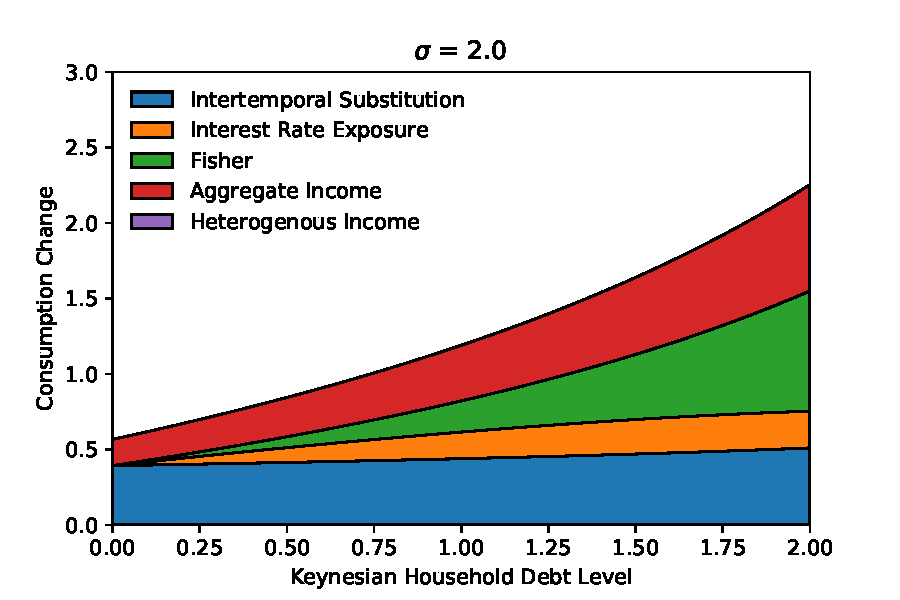
\includegraphics[width=9cm]{KeynesianDebt_sigma2_sw.pdf}\\
	}
	\only<3>{
		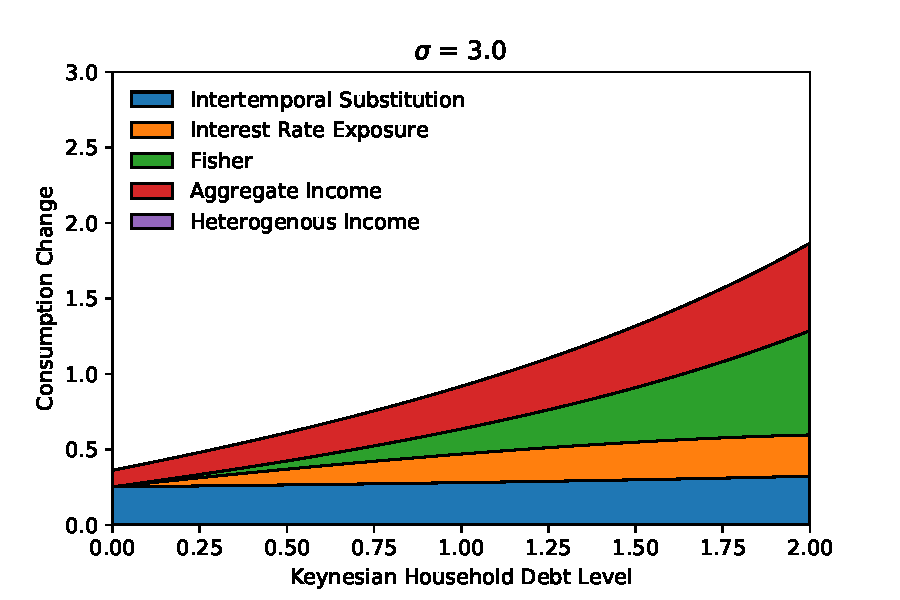
\includegraphics[width=9cm]{KeynesianDebt_sigma3_sw.pdf}\\
	}
	\only<4>{
		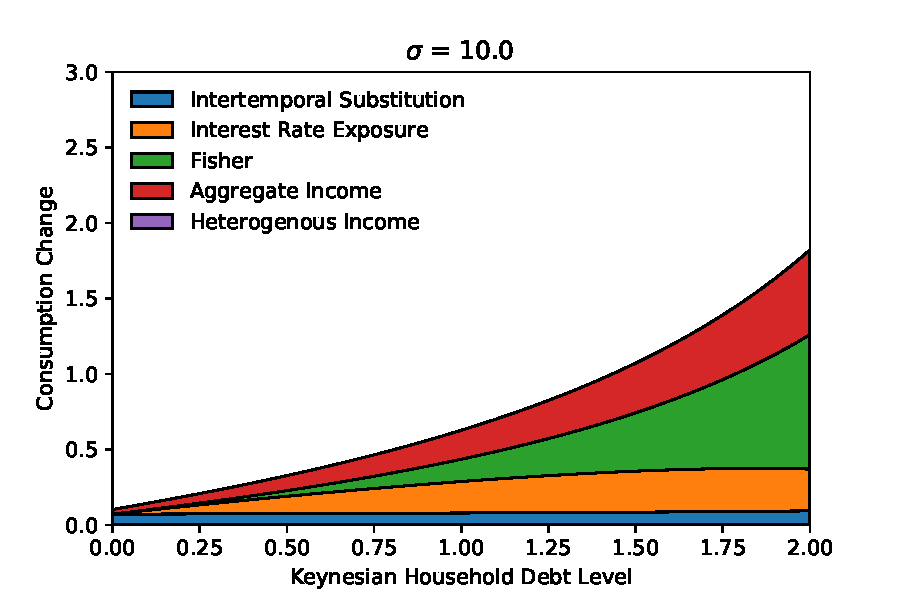
\includegraphics[width=9cm]{KeynesianDebt_sigma10_sw.pdf}\\
	}
	Intertemporal Substitution and Interest Rate Exposure act as initial `kick'\\
	Fisher and Income channels amplify this
}
\frame{
	\frametitle{Monetary Policy acts with ``Long and Variable Lags''}
	Intertemporal Subsitution doesn't give rise to a lag
	\begin{itemize}
	\item Habits - but no micro evidence
	\item Sticky Information
	\end{itemize}
	Interest Rate Exposure naturally acts wtih a lag
	\begin{itemize}
	\item 
	\end{itemize}
}
\frame{
	\frametitle{Delayed Interest Rate Exposure Response}
	\centering
	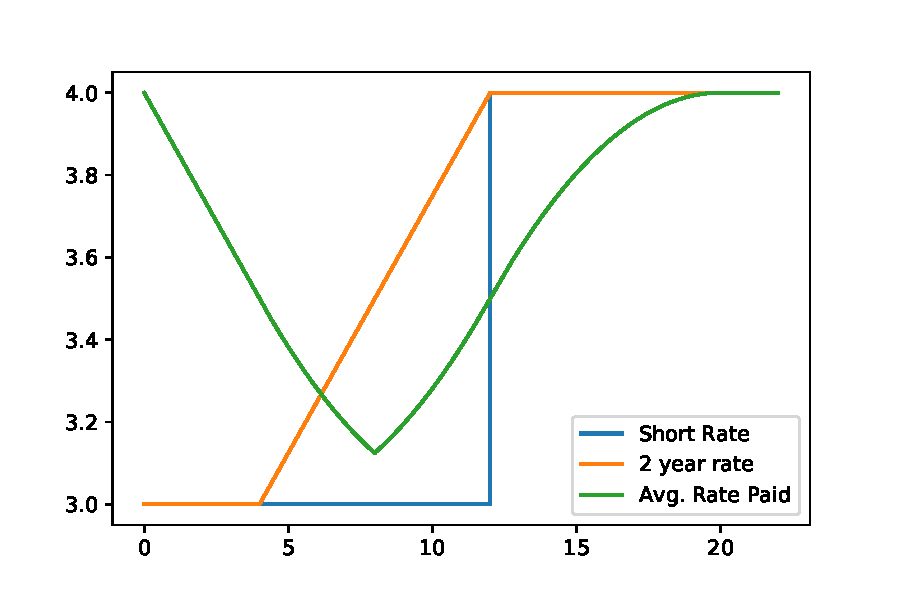
\includegraphics[width=11cm]{delayed_response.pdf}
}
\section{HANK}
\frame{
	\frametitle{Solving HANK Models is more involved}
We need new solution methods
\begin{itemize}
	\item \cite{reiter_solving_2009}
	\item Winberry (forthcoming QE)
	\item \cite{ahn_when_2017}
	\item \cite{blSolving}
\end{itemize}
\bigskip
What do we gain?
\begin{itemize}
	\item Uncertainty
	\item Matches micro behavior ???
	\item Kaplan, Moll and Violante claim transmission is very different to TANK
\end{itemize}
}
\frame{
	\frametitle{Greenwood, Hercowitz and Huffman Preferences}
	Many HANK models use GHH preferences
	\begin{align*}
	U(c,n) = u(c - \nu(n) )
	\end{align*}
	Removes wealth effects from labor decision\\
	\bigskip
	\pause
	BUT these preferences have a strong link between consumption and hours worked\\
	Extra transmission channel:
\begin{align*}
\text{GHHchannel} = \mathbb{E}\left((1-MPC_i) h_i\right)  \frac{\bar{N}}{\psi} d\omega
\end{align*}
}


\begin{comment}

\frame
{
	\frametitle{Heterogeneous Agent + New Keynesian}
	\begin{itemize}
		\item Large literature on Heterogeneous Agents
		\item Large literature on Representative Agent New Keynesian Models (RANK)
	\end{itemize}
	\pause
	Up until recently very little overlap
	\begin{itemize}
		\item B\tikzmark{start}elief heterogeneity didn't matter for monetary policy \tikzmark{end}
		\item Computational difficulties 
	\end{itemize}
	\pause
	New HANK literature shows these to be false
	
\begin{tikzpicture}[remember picture,overlay]
	\node[draw,line width=2pt,red,ellipse,inner ysep=15pt,fit={(pic cs:start) (pic cs:end)}] {};
	\end{tikzpicture}
}
\frame
{
	\frametitle{Heterogeneous Agent + New Keynesian}
	RANK model (Representative Agent NK)
	\begin{itemize}
		\item Monetary policy transmission through Intertemporal Substitution
		\item MPCs around 3\%
	\end{itemize}
\pause
	TANK model (Two Agent NK)
	\begin{itemize}
		\item High MPCs by construction
		\item Doesn't match micro behavior - but good enough for macro? \cite{dgHANKTANK}
	\end{itemize}
\pause
	HANK model (Heterogeneous Agent NK)
	\begin{itemize}
		\item Can have high MPCs (ex-ante heterogeneity in $\beta$, or illiquid asset)
		\item Matches micro behavior. Can model uncertainty shocks.
	\end{itemize}
}
\frame
{
	\frametitle{Outline for Today}
	\begin{itemize}
		\item Empirical Framework and Evidence (\cite{auclert_monetary_2017})
		\item Two Agent New Keynsian Models (TANK)
		\item Solution methods for HANK (\cite{blSolving})
	\end{itemize}
}

\section{Auclert}
\frame
{
	\frametitle{Auclert's Experiment}
	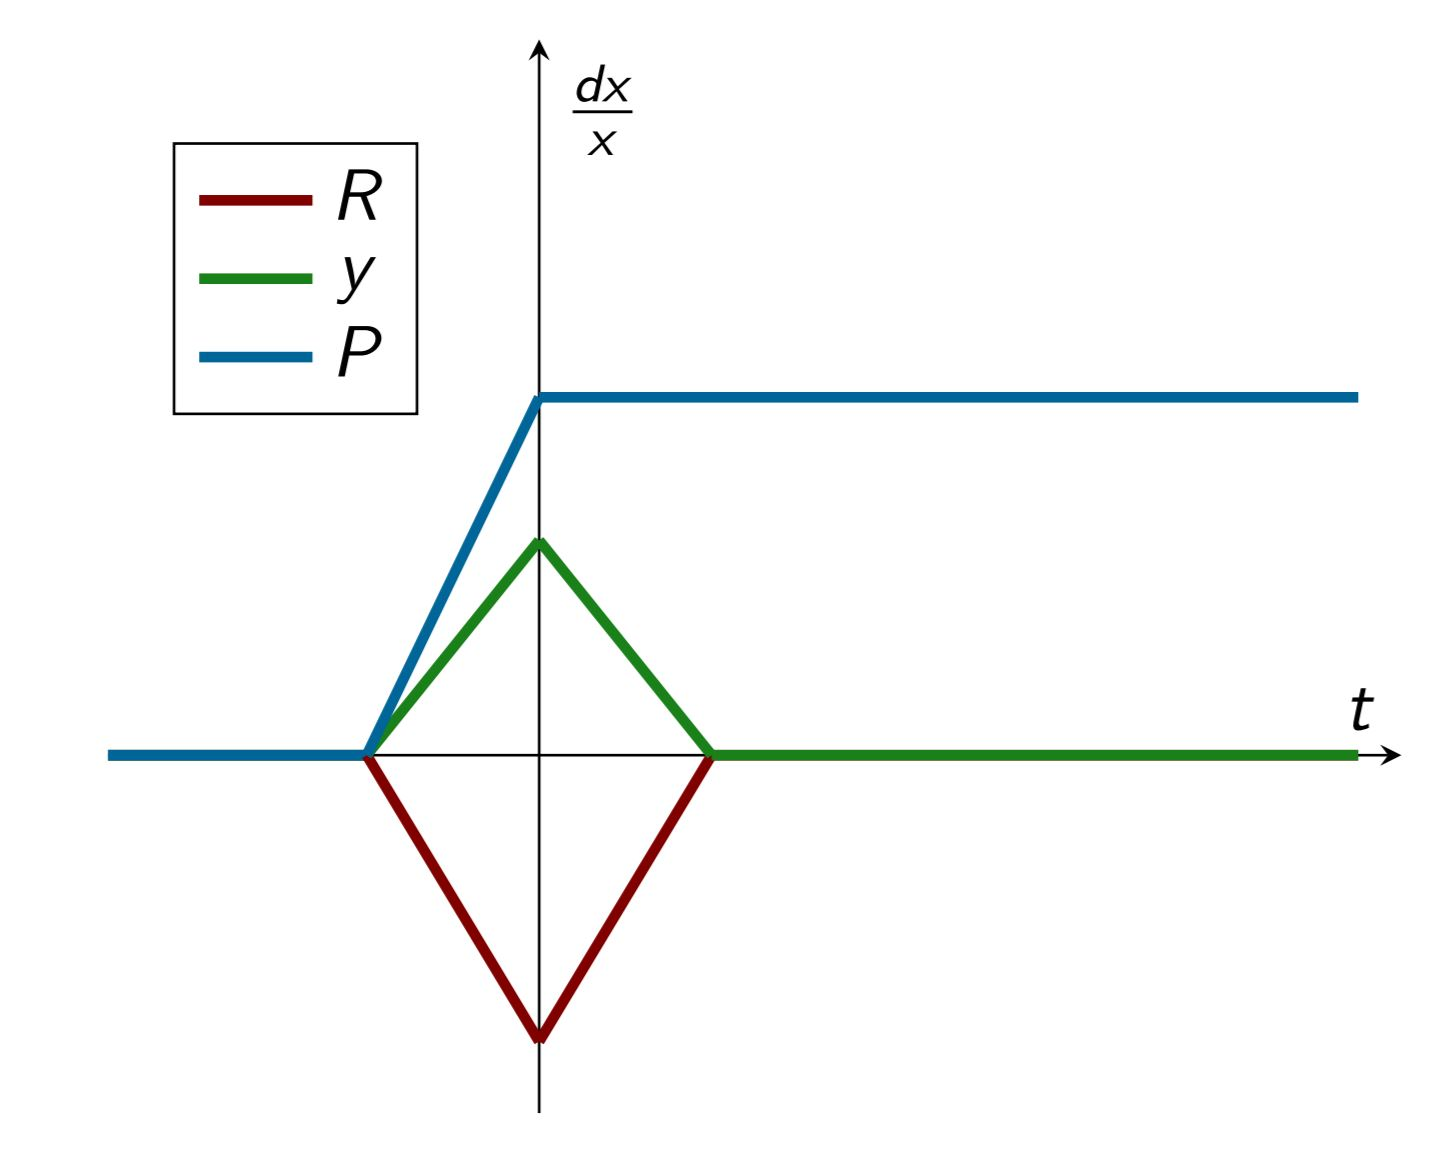
\includegraphics[width=9cm]{auclert_graph.jpg}
}

\frame
{
	\frametitle{Income Channels}
	Income for household $i$ changes $dY_i$, then
	\begin{align*}
	dC_i = \text{MPC}_i dY_i
	\end{align*}
	\pause
	Aggregate:
	\begin{align*}
	dC = \mathbb{E}_i \left(\text{MPC}_i dY_i \right)
	\end{align*}
	\pause
	Split into \textit{Aggregate Income} and \textit{Earnings Heterogeneity} channels
	\begin{align*}
	\textit{AggInc} = \mathbb{E}_i \left( \text{MPC}_i Y_i  \right) \frac{dY}{Y}
	\end{align*}
	\begin{align*}
	\textit{EarnHet} = \mathbb{E}_i \left( \text{MPC}_i dY_i  \right) - \mathbb{E}_i \left( \text{MPC}_i Y_i  \right) \frac{dY}{Y}
	\end{align*}
}
\frame{
	\frametitle{Fisher Channel}
	\textbf{Key assumption:} \\Households treat redistribution like an income shock\\
	\pause
	\bigskip
	\textbf{Experiment}
	\begin{itemize}
		\item[] One time price level increase
		\item[] Hold constant income and real interest rate
	\end{itemize}
	\bigskip
	Dimension of Redistribution: \textbf{Net Nominal Position}
	\begin{align*}
	dC_i = MPC_i NNP_i \frac{dP}{P}
	\end{align*}
	\pause
	Aggregate:
	\begin{align*}
	dC = \mathbb{E}_i \left(MPC_i NNP_i\right) \frac{dP}{P}
	\end{align*}
}
\frame{
	\frametitle{Interest Rate Exposure Channel}
	\textbf{Experiment}
	\begin{itemize}
		\item[] Short term real interest rate $\uparrow$ 1\% for 1 year
		\item[] Hold constant income and inflation
	\end{itemize}
	\bigskip
	Dimension of Redistribution: \textbf{Unhedged Interest Rate Exposure}\\
	URE Definition: Net savings made at this year's interest rate
	\begin{align*}
	URE_i = Y_i - C_i + A_i - L_i
	\end{align*}
	Where
	\begin{itemize}
		\item $Y_i = $ Total after tax income 
		\item $C_i = $ Total Expenditure, including interest payments
		\item $A_i = $ Maturing assets
		\item $L_i = $ Maturing liabilities
	\end{itemize}
	\begin{align*}
	dC_i = MPC_i URE_i  \frac{dR}{R}
	\end{align*}
}
\frame{
	\frametitle{Interest Rate Exposure Channel}
	\label{aggregation}
	Aggregate to find size of channel:
		\begin{align*}
		dC_i &= \quad \ \ MPC_i URE_i  \ \ \ \frac{dR}{R} \\
		\implies dC &= \mathbb{E}_I \Big(MPC_i URE_i   \Big) \frac{dR}{R} 
		\end{align*}
}
\frame{
	\frametitle{Evidence from Denmark}
	\begin{center}
		\begin{tikzpicture}
		\node (img2) {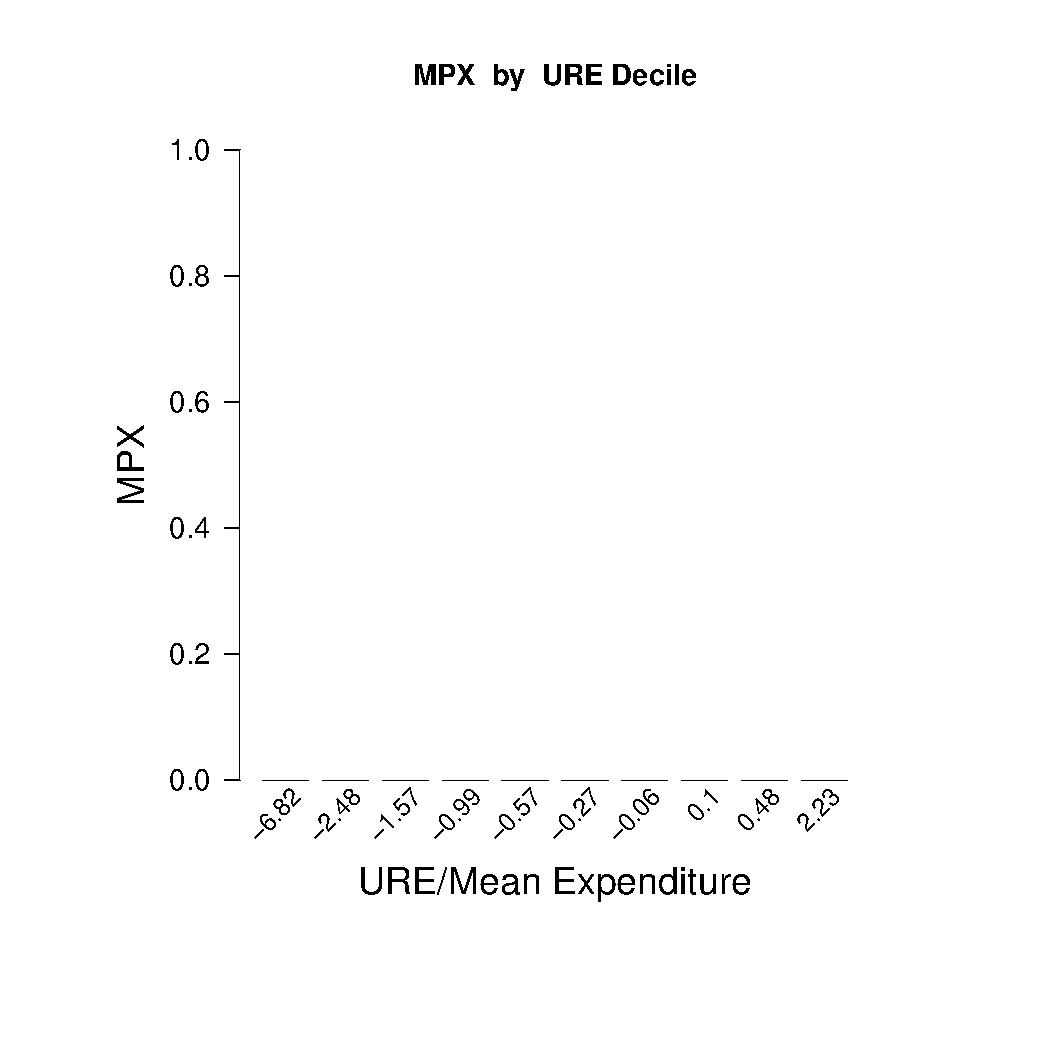
\includegraphics[scale=0.53,trim=0 0 0 1.7cm ,clip]{MPXByUREdetailsblank_level_lincome_head.pdf}};
		\node (img3)
		{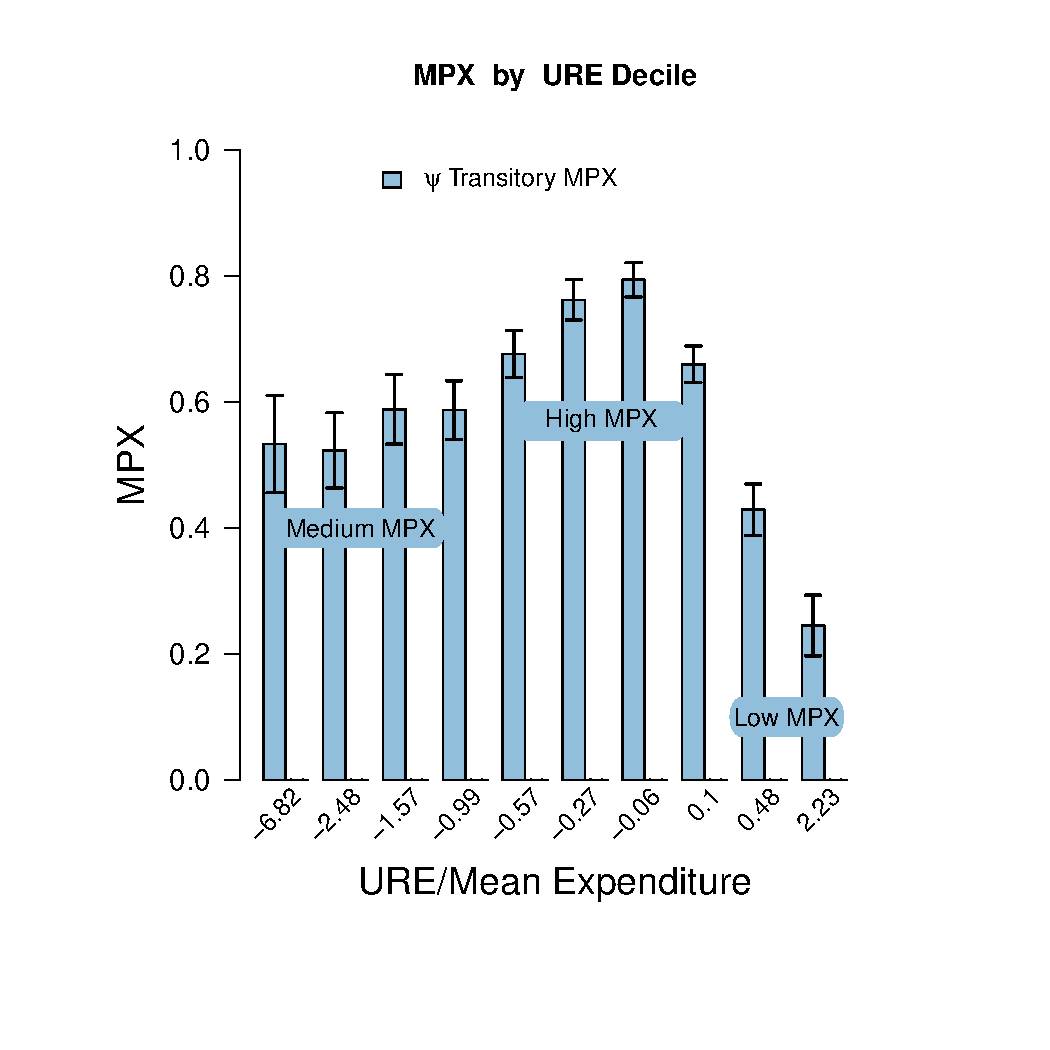
\includegraphics[scale=0.53,trim=0 0 0 1.7cm ,clip]{MPXByUREdetails1a_level_lincome_head.pdf}};
		\pause
		\node (img6) {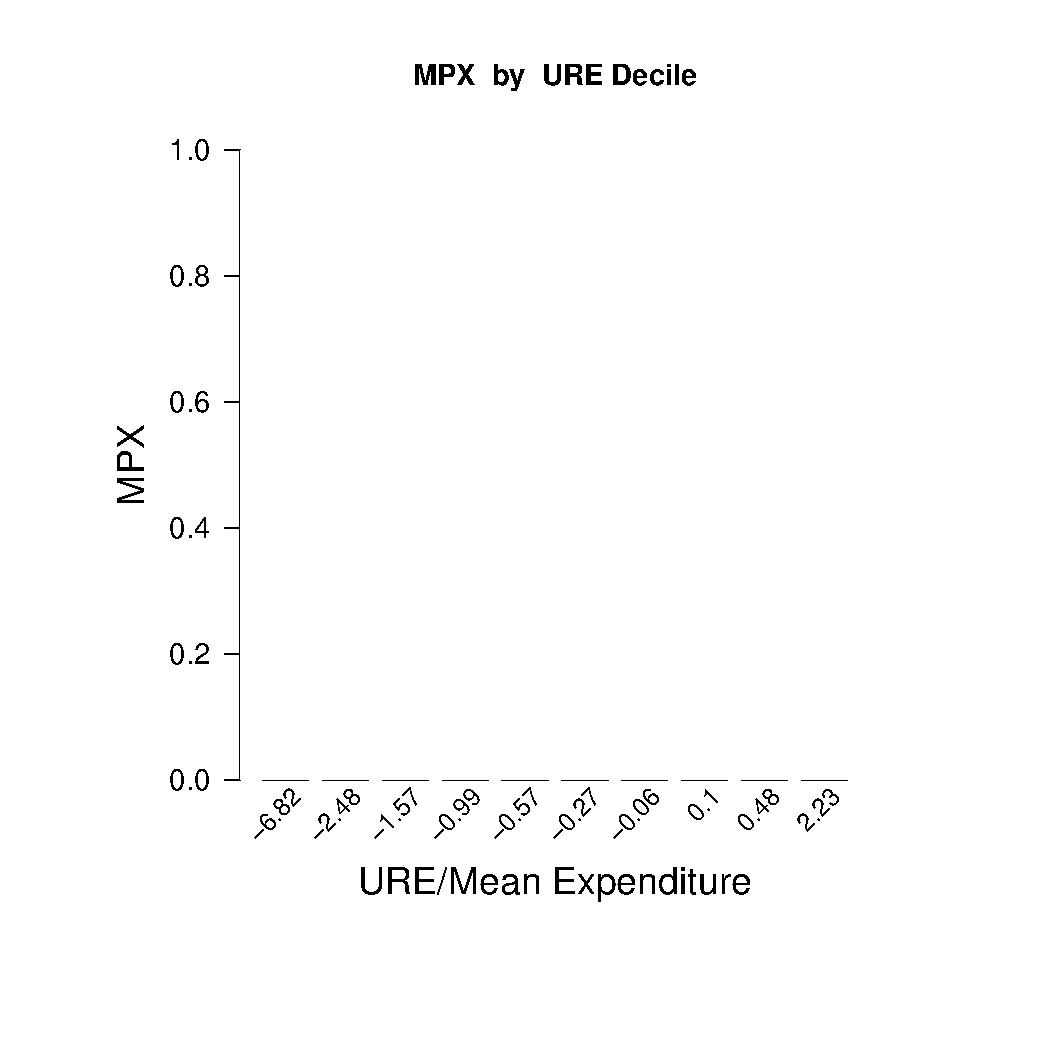
\includegraphics[scale=0.53,trim=0 0 0 1.7cm ,clip]{MPXByUREdetailsblank_level_lincome_head.pdf}};
		\node (img7)
		{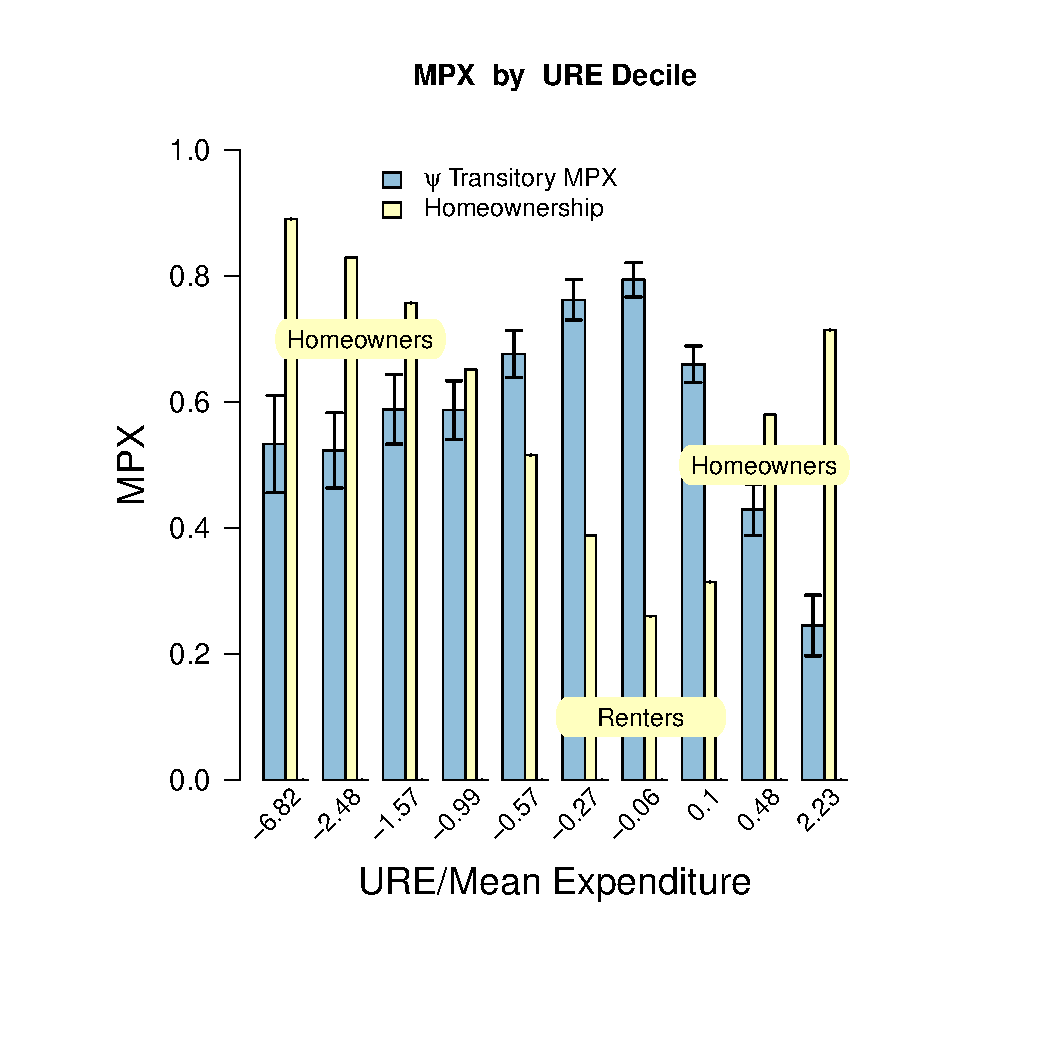
\includegraphics[scale=0.53,trim=0 0 0 1.7cm ,clip]{MPXByUREdetails2a_level_lincome_head.pdf}};
		\pause
		\node (img10) {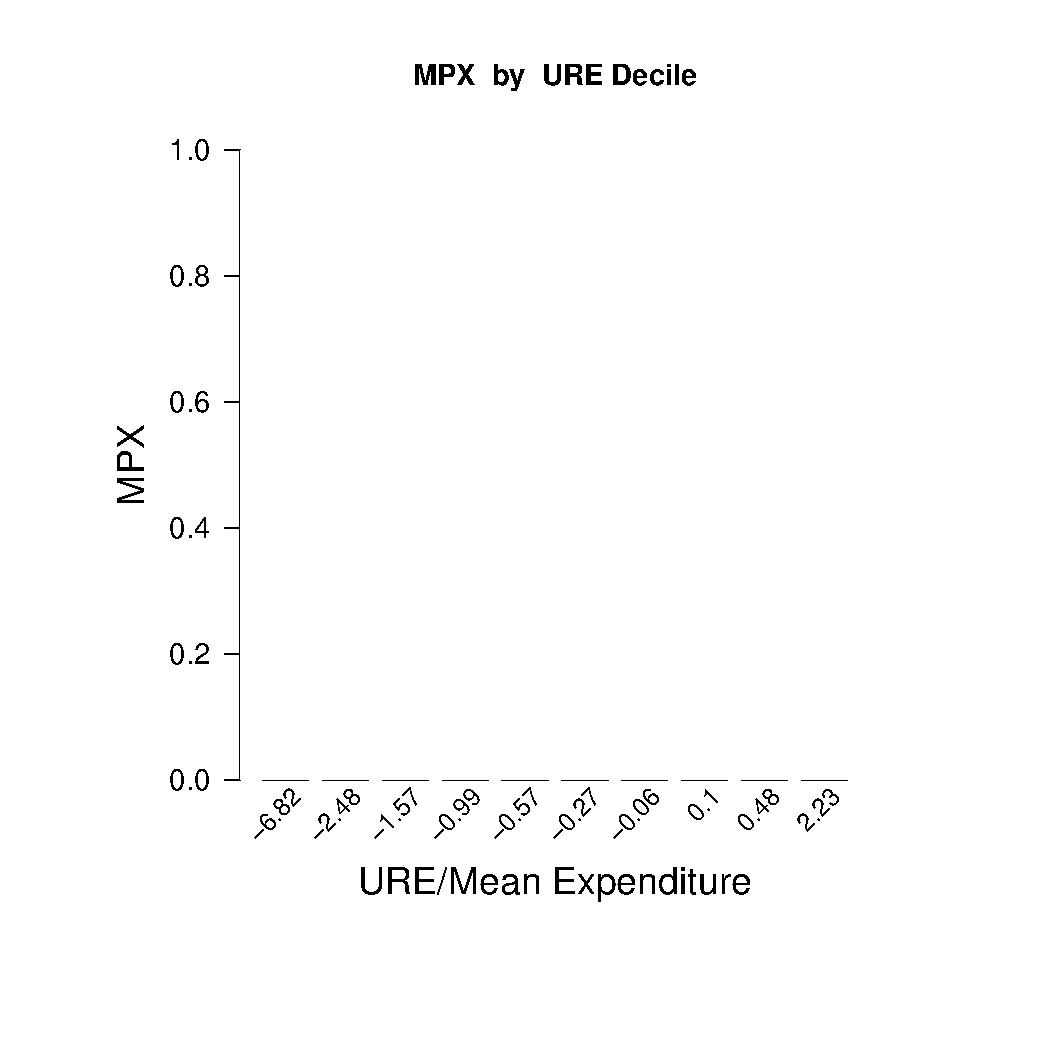
\includegraphics[scale=0.53,trim=0 0 0 1.7cm ,clip]{MPXByUREdetailsblank_level_lincome_head.pdf}};
		\node (img11) {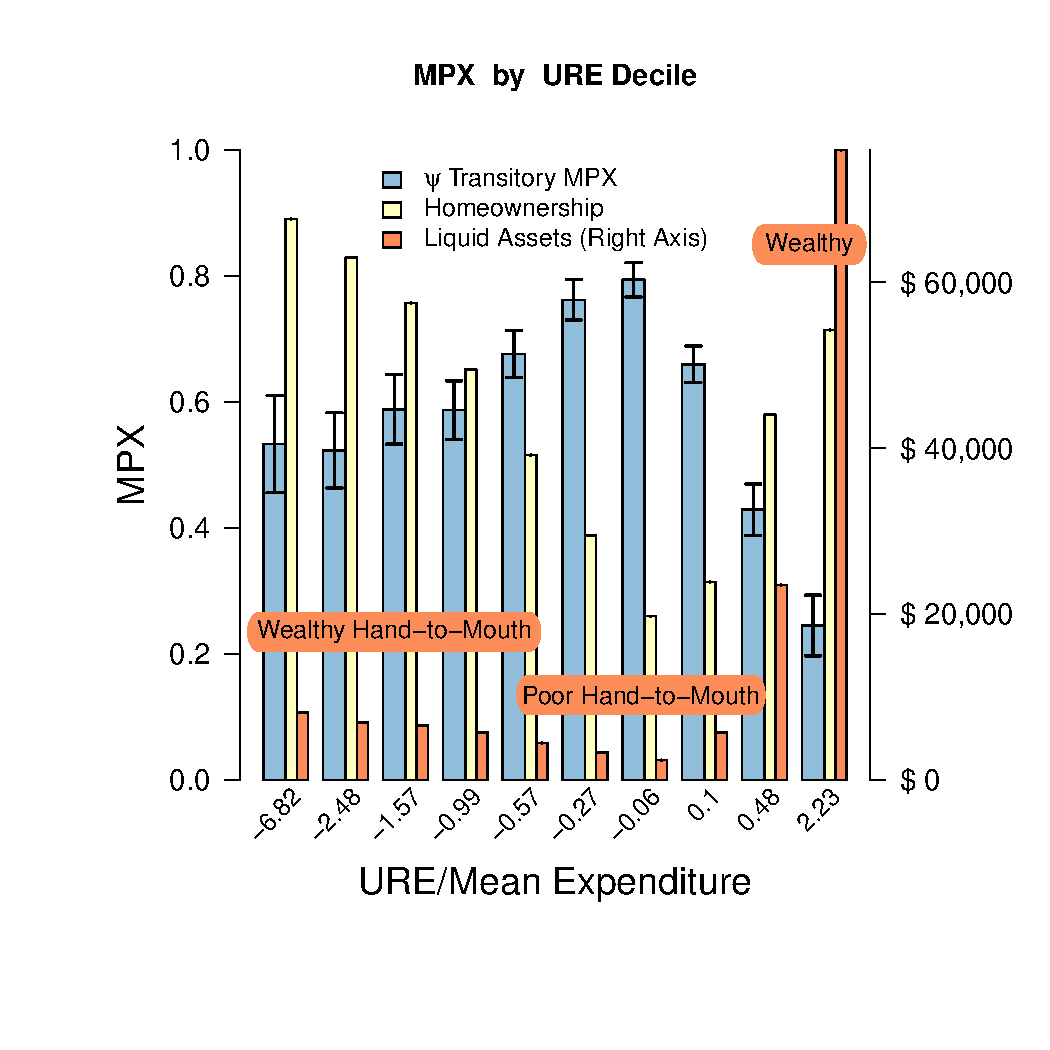
\includegraphics[scale=0.53,trim=0 0 0 1.7cm ,clip]{MPXByUREdetails3a_level_lincome_head.pdf}};
		\onslide<1->
		\end{tikzpicture}
	\end{center}
}
\frame{
	\frametitle{Intertemporal Substitution Channel}
	\begin{align*}
	dC = \mathbb{E}_i \left( \sigma_i (1-\text{MPC}_i) C_i  \right) \frac{dR}{R}
	\end{align*}
}
\frame{
	\frametitle{All Five Transmission Channels}
	\begin{align*} 
	\frac{dC}{C} &= \overbrace{\mathcal{M}\frac{dY}{Y}}^{\text{Aggregate Income Channel}\qquad} \overbrace{ + \gamma \mathcal{E}_Y \frac{dY}{Y}}^{\text{Earnings Heterogeity Channel}\qquad} \overbrace{ - \mathcal{E}_P\frac{dP}{P}}^{\text{Fisher Channel}}  \nonumber \\
	& \qquad \underbrace{ + \mathcal{E}_R \frac{dR}{R}}_{\text{Interest Rate Exposure Channel}\qquad}  \underbrace{ - \sigma \mathcal{S}\frac{dR}{R}}_{\text{Intertemporal Substitution Channel}} \label{auclert_channels}
	\end{align*}
	\begin{columns}
		\column{0.5\linewidth}
		\centering
		\input sufficient_stats2.tex
		\column{0.5\linewidth}
		\pause
		Compare $\mathcal{E}_R$ to $\sigma S$:\\
		\bigskip
		$\sigma \approx 0.1$ Best, Cloyne, Ilzetzki, and Kleven (2018)\\
		\bigskip
		$\sigma S \approx 0.05$ \\
	\end{columns}
	
	\begin{tikzpicture}[remember picture,overlay]
	\draw[red,thick] (2.84,0.87) circle (0.45cm);
	\draw[red,thick] (7.1,0.51) circle (0.45cm);
	\end{tikzpicture} 
}

\frame{
\frametitle{Some Time Series Evidence}
I have presented cross-sectional evidence\\
\bigskip
Some time series evidence:
\begin{itemize}
	\item \cite{wong_population_2016}
	\item \cite{cloyne_monetary_2016}
\end{itemize}
}
\frame{
	\frametitle{How does Investment Change Things?}
	\centering
	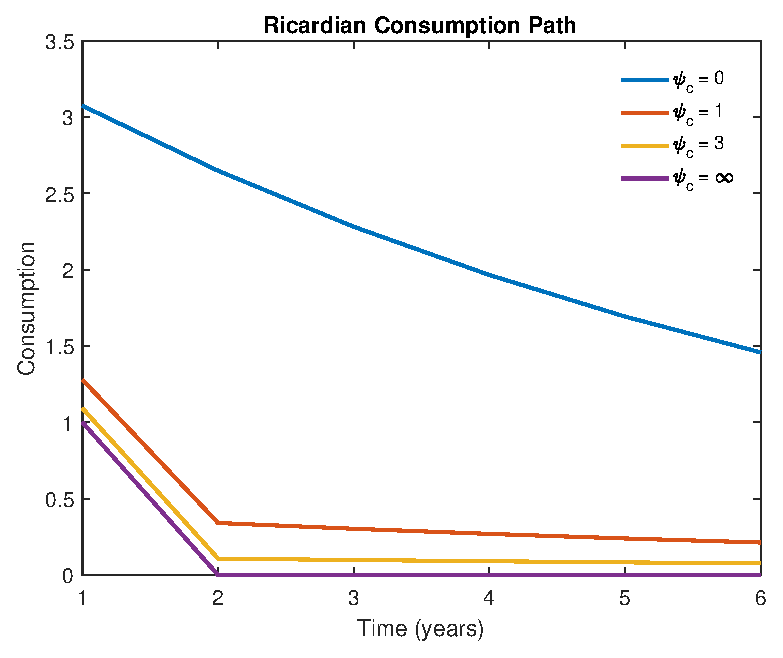
\includegraphics[scale=0.35]{TANK_capital_IRF_c_R.eps}
	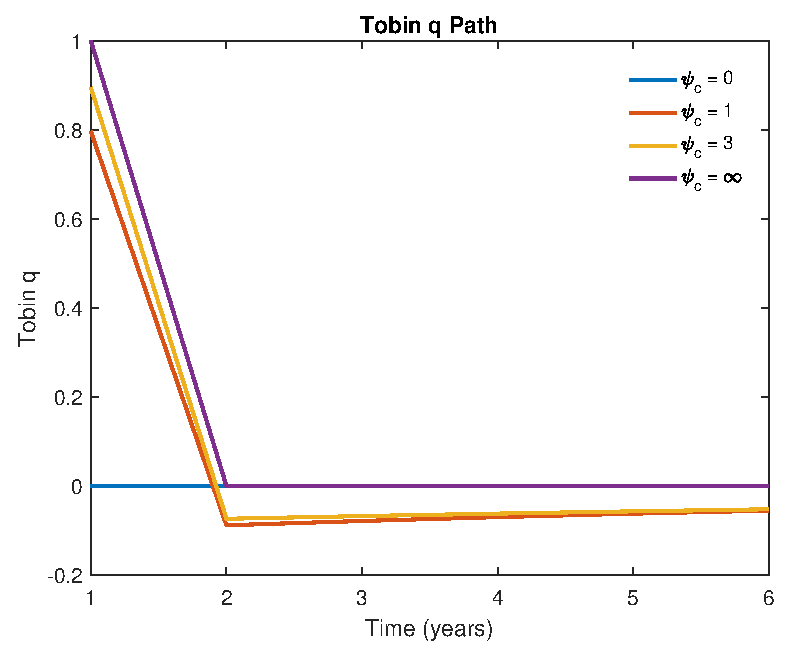
\includegraphics[scale=0.35]{TANK_capital_IRF_q.eps} \\
	Depends on Adjustment Costs $\psi_c$ \\
	Extra `kick' from firm investment
}
\section{HANK}
\frame{
	\frametitle{Solving HANK Models is more involved}
The entire distribution of wealth is a \textit{predetermined} variable\\
\bigskip
We need new solution methods
\begin{itemize}
	\item \cite{reiter_solving_2009}
	\item Winberry (forthcoming QE)
	\item \cite{ahn_when_2017}
	\item \cite{blSolving}
\end{itemize}
Bayer Luetikke code available in HARK...
}
\frame{
	\frametitle{Greenwood, Hercowitz and Huffman Preferences}
	Many HANK models use GHH preferences
	\begin{align*}
	U(c,n) = u(c - \nu(n) )
	\end{align*}
	Removes wealth effects from labor decision\\
	\bigskip
	\pause
	BUT these preferences have a strong link between consumption and hours worked\\
	Extra transmission channel:
\begin{align*}
\text{GHHchannel} = \mathbb{E}\left((1-MPC_i) h_i\right)  \frac{\bar{N}}{\psi} d\omega
\end{align*}
}

\end{comment}

%%%%%%%%%%%%%%%  bibliography

\bibliographystyle{\econtexBibStyle}
\newsavebox\mytempbib
\savebox\mytempbib{\parbox{\textwidth}{\bibliography{\econtexRoot/AllPapers}}}


\end{document}

